\section{Developer Biography}\label{chap:biography}
\vspace{-0.9em}

\begin{center}
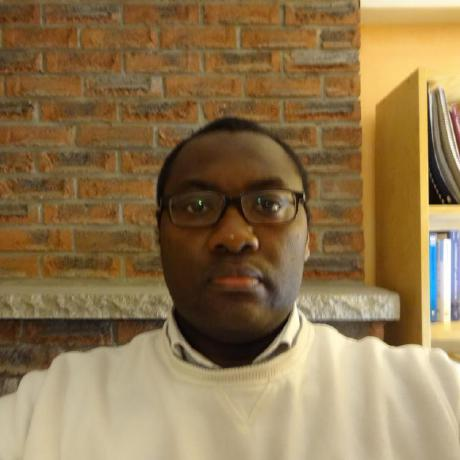
\includegraphics[scale=0.32]{../../francais/images/XavierNOUNDOU-2}
\captionof{figure}{Portrait of DR. XAVIER.\label{fig:xaviernoumbis}}
\end{center}

\textbf{\myfullacademicname} is a CHRISTIAN BY FAITH,
Cameroonian, born on September~$16$ $1983$ in
DOUALA (LITTORAL region, CAMEROON).

Xavier has a \textit{''Diplom--Informatiker (Dipl.--Inf.)''}
qualification from the \textbf{\unibremen, Bremen, Bremen, GERMANY} (May~$25$, $2007$).

Xavier is a \textit{PH.D. in Software Engineering}
(software construction, and testing) since November~$18$,~$2020$
because of his academic research, and professional engineering
contributions as follows:


\begin{enumerate}
%	\itemsep -0.7em
	\item 'Context-Sensitive Staged Static Taint Analysis
			For C using LLVM'
		\begin{enumerate}[1.]
			\itemsep -0.7em
			\item source code: \\
			\url{http://github.com/xnoumbissinoundou/yeroth-saint}
			\item full text (published on July~$1^\text{st}$, $2015$): \url{http://archive.org/details/saint_201507}.
		\end{enumerate}		 

	\item 'YEROTH-ERP-3.0':
			\begin{enumerate}[1.]
			\itemsep -0.7em
			\item source code: \\
			\url{http://github.com/xnoumbissinoundou/yeroth-erp-3.0}
			\item full text (ongoing publication): \url{http://archive.org/details/yeroth-erp-3-0-info-english}.
		\end{enumerate}	
\end{enumerate}
